\documentclass[twocolumn]{IEEEtran}
\usepackage[utf8x]{inputenc}
\usepackage{amssymb,amsfonts}
\usepackage[tbtags]{amsmath}
\usepackage{graphicx}
\usepackage{cite}
\usepackage{slashbox}
\usepackage{pict2e}
\usepackage{float}
\usepackage[all]{xy}
\usepackage{graphics,graphicx,color,colortbl}
\usepackage{times}
\usepackage{subfigure}
\usepackage{wrapfig}
\usepackage{multicol}
\usepackage{cite}
\usepackage{url}
\usepackage[tbtags]{amsmath}
\usepackage{amsmath,amssymb,amsfonts,amsbsy}
\usepackage{bm}
\usepackage{algorithm}
\usepackage{algorithmic}
\usepackage[centerlast, small]{caption}
\usepackage[colorlinks=true, citecolor=blue, linkcolor=blue, urlcolor=blue, breaklinks=true]{hyperref}
\begin{document}
\title{Circuitos acoplados magnéticamente}
\author{José Fabio Lozano Ovalle Código: $222982$\\
	Wilson Orlando Macias Fuquen Código: $223101$\\
	David Ricardo Martínez Hernández Código: $261931$}
\maketitle
\markboth{Universidad Nacional de Colombia}{}
\floatname{algorithm}{Algoritmo}
\begin{abstract}
Se realizara el montaje de un circuito acoplado magnéticamente y se hallaran experimentalmente los valores de $L_1$, $L_2$ y $M$, adicionalmente se determinara la polaridad relativa de los inductores y la relación de transformación entre primario y secundario. Por ultimo se implementara un circuito para  visualizar la curva de histéresis del núcleo de hierro utilizado para acoplar los inductores.
\end{abstract}
\begin{keywords}
Autoinductancia, Bobina, Corriente, Flujo Magnético, Histéresis, Inductancia Mutua, Magnetismo, Magnetización, Material Ferromagnético, Permeabilidad.
\end{keywords}

\section{Objetivos}
\begin{itemize}
 \item Visualizar experimentalmente el ciclo de histéresis del núcleo hierro utilizado como acople por medio del osciloscopio.
 \item Aplicar las ecuaciones de Ampere y Faraday en el planteamiento de las ecuaciones de los circuitos del sistema acoplado magnéticamente.
 \item Determinar experimentalmente los valores de $L_1$, $L_2$, $M$, y la polaridad relativa de los inductores.
 \item Comparar experimentalmente la relación de transformación entre primario y secundario, por medio del número de espiras, voltajes y corrientes.
\end{itemize}

\section{Introducción}
\noindent
Siempre que la corriente fluye a través de un conductor, ya sea $AC$ o $DC$, se genera un campo alrededor de él. En circuitos, se refiere a menudo al \textit{flujo magnético} a través de un lazo de alambre, que es la componente normal promedio del campo magnético que emana del lazo, multiplicada por el área del mismo. Cuando un campo magnético variable en el tiempo generado por un lazo penetra un segundo lazo, se induce una tensión entre los extremos de este último.\footnote{Texto tomado de \cite{hayt}, Página 491}

\section{Hipótesis}
\noindent
Se espera que la relación de transformación sea muy parecida a la razón del número de espiras entre secundario  y primario.\\
Se espera una curva de histéresis de área pequeña si el núcleo no se calienta demasiado, de lo contrario se tendría una curva un poco mas ancha.

\section{Materiales}
\begin{itemize}
 \item Bobinas
 \item Condensador de $1\ \ \mu F$
 \item Multímetro
 \item Núcleo de un material Ferromagnético
 \item Osciloscopio
 \item Resistencias
\end{itemize}

\section{Análisis Y Resultados}
\noindent
Para esta práctica se implementaran 2 circuitos monofásico para analizar en estos el fenómeno de acoplamiento magnético.

\subsection{Circuito con transformador}
\noindent
Para este circuito se tiene una fuente AC que alimenta el primario y en el secundario se tiene un circuito abierto para analizar la tensión en cada uno y obtener la ganancia del transformador.
\begin{figure}[H]
	\centering
		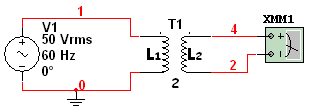
\includegraphics[scale=0.7]{circ1.PNG}
	\caption{Circuito monofásico con transformador.}
	\label{fig10}
\end{figure}
\noindent
Para la parte práctica se obtuvo los siguientes datos: número de vueltas en el primario $N_1= 250$, en el secundario $N_2 = 500$.\\
El voltaje de entrada que se obtuvo al realizar el circuito fue de $V_{IN} = 59\ V$, el voltaje de salida que se obtuvo fue de $V_{OUT} = 112\ V$, la corriente en el primario fue de $I_1 = 4.44\ A$, la corriente en el secundario fue de $I_2 = 2.093\ A$.
\begin{figure}[H]
	\centering
		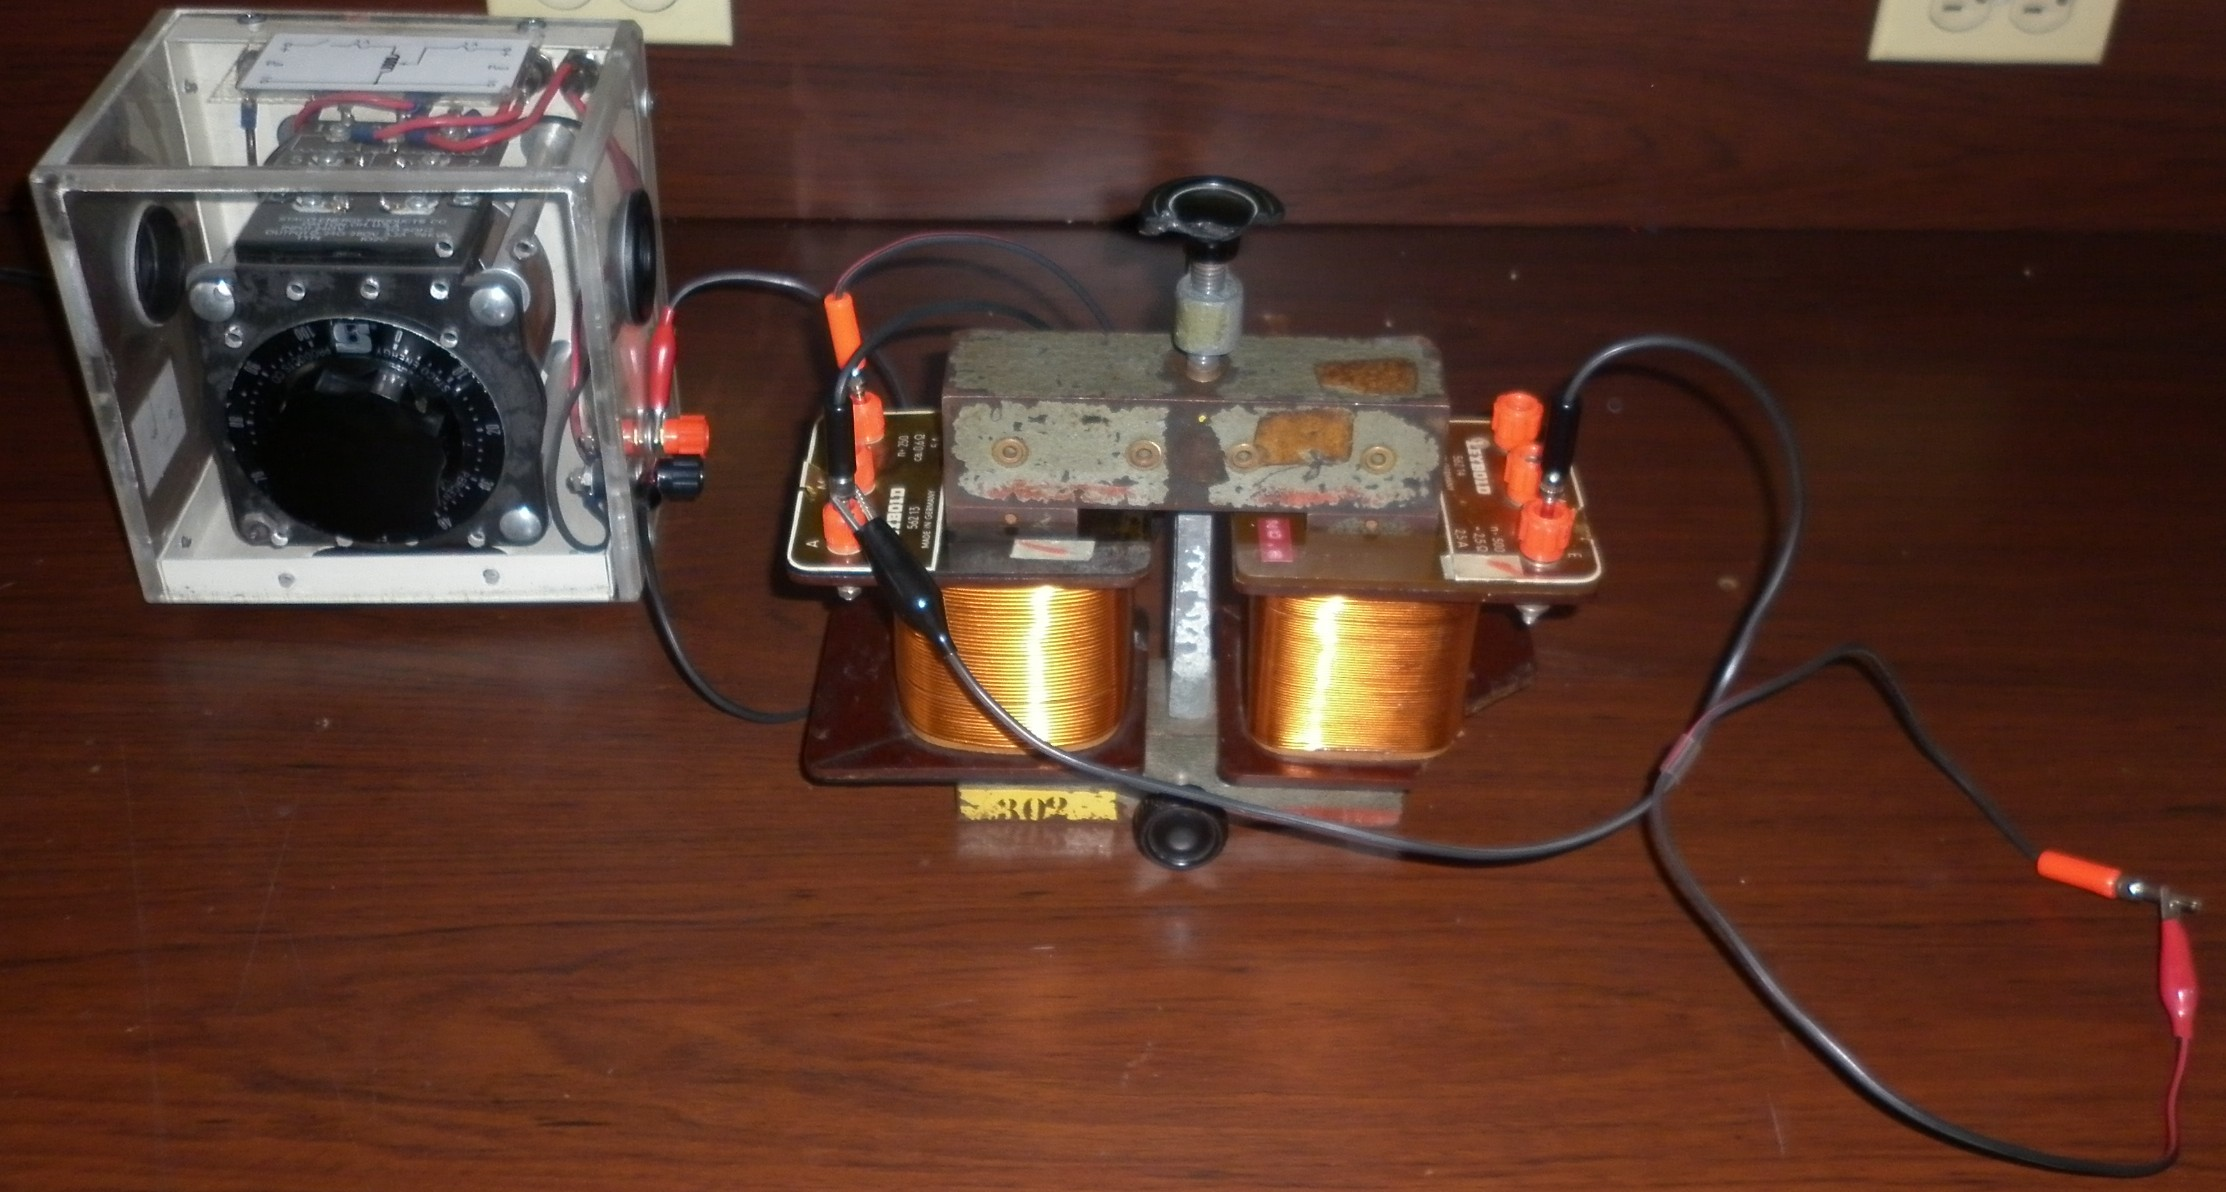
\includegraphics[scale=0.12]{436.png}
	\caption{Circuito monofásico con transformador realizado en el laboratorio}
	\label{fig20}
\end{figure}

\subsubsection{Relación de transformación}
\noindent
Para este circuito se hizo una variación en la parte práctica, con lo en análisis teórico arroja los siguientes resultados: una tensión en  $L_1$ de $V_1$=60[V], y en $L_2$ un $V_2$=120[V]aproximadamente, con estos datos se obtiene una relación de transformación debido a la tensión en el primario con respecto secundario.
\begin{equation}
 m =  \frac{V_2}{V_1}=\frac{120\ [V]}{60\ [V]}=2
\label{ecu30}
\end{equation}
\noindent
Esto se comprueba  en la práctica con la relación en el número de espiras en cada embobinado así:
\begin{equation}
 m =  \frac{N_2}{N_1}
\label{ecu31}
\end{equation}
\noindent
Con los datos obtenidos en la parte práctica se obtienen los siguientes resultados.
\begin{equation}
 m =  \frac{V_2}{V_1}=\frac{112[V]}{59[V]}=1.8983
\label{ecu10}
\end{equation}
\begin{equation}
 m =  \frac{N_2}{N_1}=\frac{500}{250}=2
\label{ecu11}
\end{equation}
\noindent
Finalmente se puede observar que el $M$ obtenido en la ecu. (\ref{ecu10}) es aproximado a los valores obtenidos en las ecu. (\ref{ecu30}) y (\ref{ecu11}).
\begin{figure}[H]
	\centering
		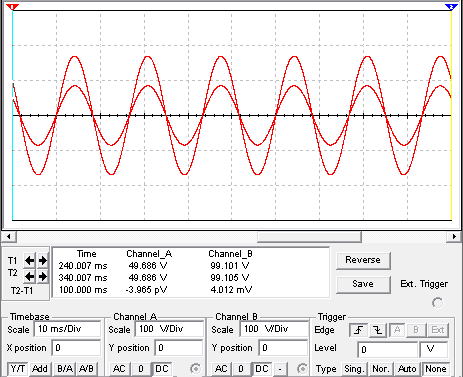
\includegraphics[scale=0.5]{sim2.PNG}
	\caption{Señal obtenida en primario y secundario.}
	\label{fig14}
\end{figure}

\subsubsection{Procedimiento para calcular inductancias $L_1$, $L_2$ y $M$}
Para obtener los valores de $L_1$, $L_2$ y $M$ se tiene datos como la corriente $i_1(T)$ y sabiendo que:
\begin{equation}
 V_1=jwL_1i_1
\label{ecu50}
\end{equation}
\noindent
Donde se despeja y se obtiene:
\begin{equation}
 L_1=|\frac{V_1}{jw i_1}|
\label{ecu51}
\end{equation}
\noindent
De igual manera se puede tener obtener $L_2$ intercambiando la energización de la fuente $AC$ o usando la ecuación de la malla en el secundario así:
\begin{equation}
 {L_2} = |\frac {V_2-j\omega M{i_1}}{j\omega {i_2} }|
\label{equ13}
\end{equation}
\noindent
Además M se obtiene así:
\begin{equation}
 M=|\frac{V_2}{jw i_1}|
\label{ecu52}
\end{equation}
\noindent
El valor calculado de $L_1$ y $L_2$ es $L_1 =35.25\ [mH]$, $L_2 =200.7\ [mH]$, por lo tanto el valor de $M$ es $M =66.91\ [mH]$.

\subsubsection{Procedimiento para hallar la polaridad relativa de los devanados primario y secundario}
\noindent
Para esta parte se debe hacer un cambio en el circuito original, se debe hacer una conexión entre las tierras de los circuitos acoplados magnéticamente, este circuito queda así:
\begin{figure}[H]
	\centering
		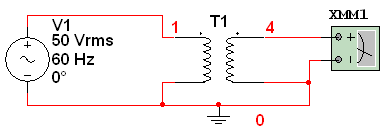
\includegraphics[scale=0.6]{circ3.PNG}
	\caption{Circuito para polaridad relativa.}
	\label{fig12}
\end{figure}
\noindent
Luego se mide la tensión entre los puntos restantes, en el circuito de la Fig.\ref{fig12} entre los puntos 1 y 4, a esta tensión se le llamara $V_M$, si se tiene que
\begin{equation}
 V_M=V_1+V_2
\label{ecu54}
\end{equation}
\noindent
La polaridad de los devanados, es decir la convención de punto es tal como está en el circuito de la Fig.\ref{fig10} y que es aditiva, si no, entonces se tiene que
\begin{equation}
 V_M=V_1-V_2
\label{ecu53}
\end{equation}
\noindent
Y la polaridad del circuito es diferente, en el segundo devanado el punto se ubica en el otro extremo, además en este caso es sustractiva.\\\\
De acuerdo al procedimiento anterior el voltaje que dio entre las bobinas fue de $V_M = 54\ V$, este voltaje se obtuvo midiendo las terminales $E_{11}$ y $A_{21}$ de la Fig. \ref{fig21}\\
\begin{figure}[H]
	\centering
		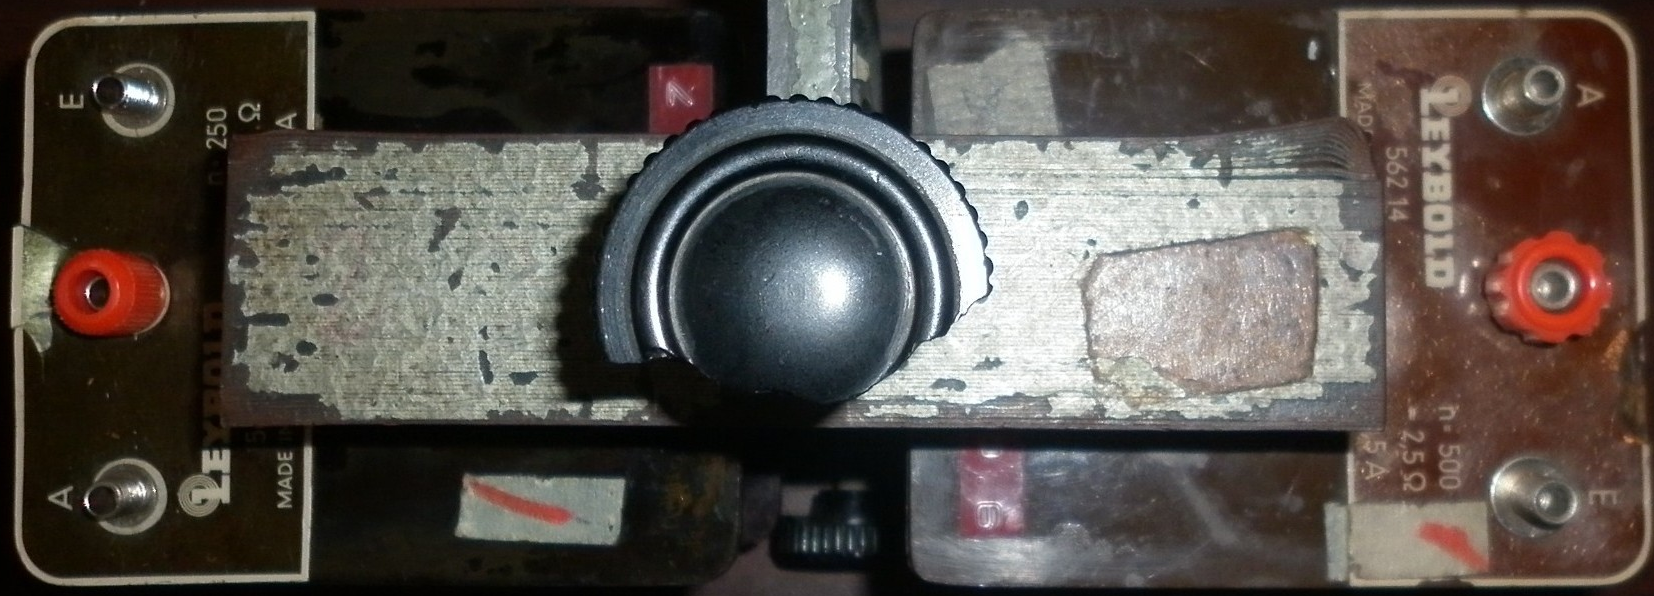
\includegraphics[scale=0.15]{432.png}
	\caption{Circuito para calcular la polaridad relativa realizado en el laboratorio}
	\label{fig21}
\end{figure}
\noindent
Para ver que polaridad se hacen las calculan los posibles resultados de $V_M$:
\begin{equation}
{V_M}=V_1-V_2=59-112=-53[V]
\label{ecu14}
\end{equation}
\begin{equation}
{V_M}=V_1+V_2=59+112=171 [V]
\label{ecu15}
\end{equation}
\noindent
De estas dos opciones, se observa que la ecu. (\ref {ecu14}) es la que más se aproxima al valor medido, dado que estos son valores $RMS$ el signo no tiene relevancia  en este cálculo. Finalmente se puede decir que la polaridad del circuito es sustractiva.

\subsection{Circuito para obtener curva de histéresis}
Para obtener la curva de histéresis del núcleo en el transformador, en este caso un material ferromagnético, se diseña el siguiente circuito.
\begin{figure}[H]
	\centering
		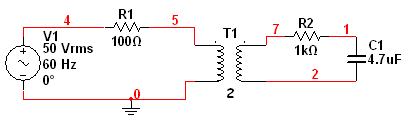
\includegraphics[scale=0.6]{circ2.PNG}
	\caption{Circuito para obtener curva de histéresis.}
	\label{fig11}
\end{figure}
\noindent
Para obtener la curva se tiene que la tensión en el condensador es
\begin{equation}
V_c(t)=\frac{1}{C}\displaystyle\int_{0}^{t} i_c(\tau)\, d\tau
\label{ecu32}
\end{equation}
\noindent
Donde $i_c(t)$ es la corriente en $R_2$ y $L_2$, entonces se tiene:
\begin{equation}
i_c(t)=\frac{V_2(t)}{R_2}
\label{ecu33}
\end{equation}
\noindent
Donde $V_2(t)$ es la tensión en el secundario, además con la ley de Faraday se puede relacionar esta tensión con el flujo en el núcleo:
\begin{equation}
V_2(t)=N_2\frac{d \phi(t)}{dt}
\label{ecu34}
\end{equation}
\noindent
Recordando que:
\begin{equation}
\phi(t)=A B(t)
\label{ecu35}
\end{equation}
\noindent
Así se obtiene que la tensión en el secundario está dada por:
\begin{equation}
V_2(t)=AN_2\frac{dB(t)}{dt}=i_c(t)R_2
\label{ecu36}
\end{equation}
\noindent
Reemplazando en la ecu. (\ref{ecu32}) se obtiene que:
\begin{equation}
V_c(t)=\frac{AN_2}{CR_2}\displaystyle\int_{0}^{t} \frac{dB(\tau)}{d\tau}\, d\tau=\frac{AN_2B(\tau)}{CR_2}\
\label{ecu37}
\end{equation}
\noindent
De donde podemos obtener $B(t)$ de forma indirecta:
\begin{equation}
B(t)=\frac{CR_2 V_c(t)}{AN_2}
\label{ecu38}
\end{equation}
\noindent
Ahora, $H(t)$ se obtiene a partir de la ley de Ampere:
\begin{equation}
\displaystyle\oint_{C} H(t)\, dl=H(t)l_m=N_1i_1(t)
\label{ecu39}
\end{equation}
\noindent
Despejando $H(t)$ se obtiene
\begin{equation}
H(t)=\frac{N_1i_1(t)}{l_m}
\label{ecu40}
\end{equation}
\noindent
Además, se sabe que la corriente  $i_1$, del primario es:
\begin{equation}
i_1(t)=\frac{V_{R1}}{R_1}
\label{ecu41}
\end{equation}
\noindent
Así se obtiene finalmente:
\begin{equation}
H(t)=\frac{N_1V_{R1}}{R_1l_m}
\label{ecu42}
\end{equation}
\noindent
Se puede observar en la ecu. (\ref{ecu38}) y (\ref{ecu42}) que $B(t)$ y $H(t)$ dependen de $V_c(t)$ y $V_{R1}$ respectivamente, además de un valor contante dado por las características del circuito, midiendo la tensión de estos elementos con un osciloscopio y programándolo en la forma $XY$ se obtendrá finalmente la curva de histéresis.\\\\
La curva que se obtuvo en el laboratorio es la Fig. \ref{fig22}.
\begin{figure}[H]
	\centering
		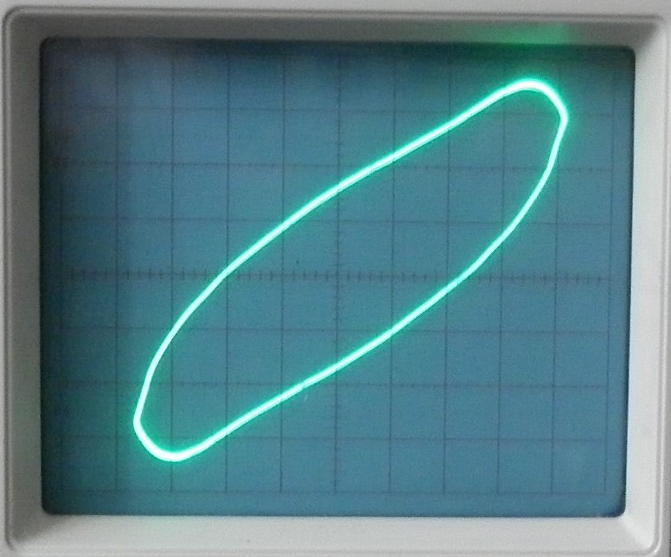
\includegraphics[scale=0.3]{445.png}
	\caption{Curva de histéresis para el montaje, vista desde el Osciloscopio}
	\label{fig22}
\end{figure}
\begin{figure}[H]
	\centering
		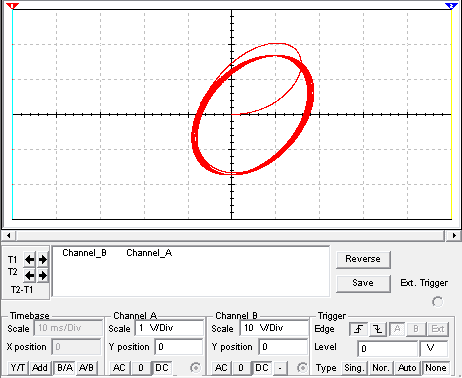
\includegraphics[scale=0.5]{sim1.PNG}
	\caption{Simulación de curva de histéresis aproximada.}
	\label{fig15}
\end{figure}

\section{Preguntas}
\begin{enumerate}
 \item ¿Como se pueden hallar los valores de $L$ y $M$ en una inductancia a partir de $V$ e $I$?\\
Para calcular los valores de $L_1$, $L_2$ y $M$ en el circuito utilizando las mediciones de corriente y voltaje montamos el siguiente circuito, donde el secundario permanece abierto Fig. \ref{fig99}.
\begin{figure}[H]
	\centering
		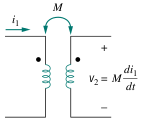
\includegraphics[scale=0.8]{pointsa.png}
	\caption{Convención de puntos}
	\label{fig99}
\end{figure}
\noindent
De la malla del circuito dos en el dominio de la frecuencia obtenemos la ecuación:
\begin{equation}
 V_2 = j \omega Mi_1
\label{equ1}
\end{equation}
\noindent
Donde podemos despejar el valor de M ya que conocemos $i_1$ y $V_2$.
Ahora realizando la malla del circuito uno en el dominio de la frecuencia obtenemos:
\begin{equation}
 {V_1} = j\omega {L_1}{i_1} + j\omega M{i_2}
\label{equ2}
\end{equation}
\noindent
Como la corriente $i_2$ es cero entonces el valor de $L_1$ se puede calcular fácilmente de la expresión:
\begin{equation}
 {V_1} = j\omega {L_1}{i_1}
\label{equ3}
\end{equation}
\noindent
Por ultimo para encontrar el valor de $L_2$ cerramos el circuito para obtener la malla:
\begin{equation}
 {V_2} = j\omega {L_2}{i_2} + j\omega M{i_1}
\label{equ4}
\end{equation}
\noindent
Donde ya son conocidos todos los valores, entonces podemos despejar $L_2$

 \item ¿Como se aplica la ley de Ampere y la ley de Faraday a un circuito de acoplamiento magnético?\\
En un circuito acoplado magnéticamente donde circula una corriente $i_1$ y el inductor $L_1$ tiene $N$ espiras, longitud $l$ y área $S$. Aplicando la ley de Ampere podemos hallar el flujo magnético en la bobina $L_1$, multiplicando el campo magnético por el área $S$:
\begin{equation}
{\Phi _1} = S{B_1} = \frac{{{\mu _0}NS{i_1}}}{l}
\label{equ5}
\end{equation}
\noindent
Si las dos bobinas tienen la misma área $S$ el flujo magnético que pasa por la segunda bobina es el mismo que genera la primera.\\
Podemos hallar el coeficiente $M$ de inducción mutua, que es la relación del flujo que pasa por la segunda bobina y la corriente que pasa por la primera.
\begin{equation}
 M = \frac{{{\Phi _2}}}{{{i_1}}} = \frac{{{\mu _0}NS}}{l}
\label{equ6}
\end{equation}
\noindent
Aplicando la ley de Faraday para cuando la corriente $i_1$ varia en el tiempo se induce una $FEM$ en el circuito dos, que la podemos hallar derivando el flujo que atraviesa la bobina $L_2$, así hallamos $V_2$:
\begin{equation}
 {V_2} =  - \frac{{d{\Phi _2}}}{{dt}} =  - M\frac{{d{i_1}}}{{dt}}
\label{equ7}
\end{equation}

 \item ¿Que es la histéresis de un material ferromagnético y como se puede observar?\\
El ciclo de histéresis de un material ferromagnético se presenta cuando un campo magnético variable en el tiempo que puede ser generado por una corriente alterna sobre un inductor,  atraviesa el material, haciendo que sus dominios magnéticos estén en constante movimiento, ya que tienden a orientarse en la dirección del campo magnético inducido por la bobina. Representando el campo magnético en función de la densidad de campo magnético (que es proporcional a la corriente), obtenemos la curva de histéresis para un material ferromagnético.
\begin{figure}[H]
	\centering
		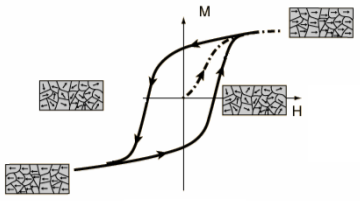
\includegraphics[scale=0.5]{pre3a.png}
	\caption{Curva de Histéresis}
	\label{fig100}
\end{figure}
\noindent
Para observar la curva de histéresis podemos utilizar un osciloscopio de dos canales en el modo $XY$, a continuación se muestra la conexión.
\begin{figure}[H]
	\centering
		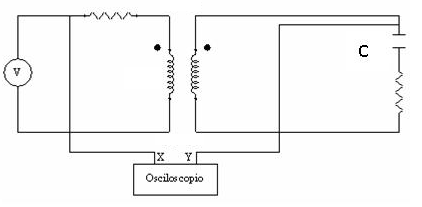
\includegraphics[scale=0.5]{pre3b.png}
	\caption{Conexión con el osciloscopio para visualizar la curva de histéresis}
	\label{fig101}
\end{figure}
\noindent
Donde  el voltaje  medido en $X$ es proporcional a la intensidad de campo magnético y el voltaje medido en $Y$ es proporcional a la densidad de flujo magnético.
\end{enumerate}

\section{Conclusiones}
\begin{itemize}
 \item La intensidad de campo magnético $H$ es proporcional a $I$ en un circuito acoplado y la densidad de flujo $B$ es proporcional a al flujo $\Phi$. Los materiales ferromagnéticos son no lineales, la magnetización máxima se alcanza con un nivel determinado de $H$, luego de alcanzar dicho valor se satura.
 \item Para poder medir la relación de transformación es necesario hacerlo en vació, si se conecta una carga en el secundario esta relación se pierde.
 \item La relación de transformación experimental no coincidió con el valor teórico debido a que parte del flujo total se perdida por flujos dispersos (Flujos externos) y las perdidas en el núcleo de hierro por corrientes parásitas y calentamiento del núcleo.
 \item No se tuvo acceso al puente Phillips (se encuentra extraviado) dado que es preciso y exacto, en este caso se comportaría como el valor teórico a comparar.
\end{itemize}

\bibliographystyle{ieeetran}
\begin{thebibliography}{99}
\bibitem{sadiku} Alexander, Charles K. \&  Sadiku, Matthew N.O.
{\em ```Fundamentals of Electric Circuits"'}.
McGRAW-HILL, ISE Editions, 1999.

\bibitem{dorf} Dorf  \& Svoboda.
{\em ```Circuitos Eléctricos"'}.
Alfaomega, Sexta Edición, 2006.

\bibitem{hayt} Hayt, William H. Jr., Kemmerly, Jack E. \& Durbin, Steven M.
{\em ```Análisis de circuitos en ingeniería"'}.
McGRAW-HILL, Séptima Edición, 2007.

\bibitem{nahvi} Nahvi, Mahmood \& Edminister, Joseph A.
{\em ```Theory and Problems of Electric Circuits"'}.
McGRAW-HILL, Fourth Edition, 2003.

\end{thebibliography}
\end{document}